% topic3.tex -- Topic 3: Electromagnetic induction, Q37-54.
\topictitle{Topic 3 - Electromagnetic Induction}

% ---- Q37 (flux with the field at an angle)
\begin{quizq}{}
A flat loop of area \qty{0.050}{m^2} is in a uniform magnetic field of \qty{0.40}{T}. The field makes an
angle of \ang{30} with the \emph{plane} of the loop. What is the magnetic flux through the loop?
\opts{\qty{0}{Wb}}{\qty{0.010}{Wb}}{\qty{0.017}{Wb}}{\qty{0.020}{Wb}}
\end{quizq}

% ---- Q38 (what does not change the flux)
\Needspace{14\baselineskip}
\begin{quizq}{}
A flat loop of wire is in a uniform magnetic field, with its plane at right angles to the field. Which
action would NOT change the magnetic flux through the loop?
\opts{Increasing the strength of the field}{Rotating the loop so that its plane is at \ang{45} to the
  field}{Squashing the loop so that its area becomes smaller}{Moving the loop sideways without rotating
  it, while it stays inside the uniform field}
\end{quizq}

% ---- Q39 (Faraday's law calculation)
\Needspace{12\baselineskip}
\begin{quizq}{}
A coil of 250 turns, each of area \qty{4.0e-3}{m^2}, is at right angles to a magnetic field of
\qty{0.60}{T}. The field is reduced steadily to zero in \qty{0.050}{s}. What is the size of the average
induced emf?
\opts{\qty{0.048}{V}}{\qty{0.60}{V}}{\qty{12}{V}}{\qty{3.0e3}{V}}
\end{quizq}

% ---- Q40 (emf graph from a flux graph)
% Flux rises 0-2 s, constant 2-3 s, falls to zero 3-4 s (twice as fast). emf = -N dPhi/dt.
% Option graphs use 0.6 units per second.
\Needspace{42\baselineskip}
\begin{quizq}{}
The graph shows how the magnetic flux $\Phi$ through a coil changes with time.
\begin{center}
  \begin{tikzpicture}
    \draw[axisline] (0,0) -- (4.6,0) node[right, font=\small] {$t$ (\si{s})};
    \draw[axisline] (0,0) -- (0,1.9) node[above, font=\small] {$\Phi$};
    \draw[line width=1.1pt] (0,0) -- (2,1.4) -- (3,1.4) -- (4,0) -- (4.4,0);
    \foreach \x in {1,2,3,4} {\draw (\x,0.06) -- (\x,-0.06) node[below, font=\footnotesize] {\x};}
  \end{tikzpicture}
\end{center}
Which graph best shows the induced emf $\varepsilon$ in the coil? (Use $\varepsilon = -N\dfrac{\Delta\Phi}{\Delta t}$.)
\gridopts{%
  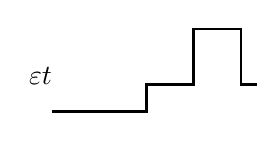
\begin{tikzpicture}\gaxesPN{$\varepsilon$}{$t$}
    \draw[line width=1pt] (0,-0.35) -- (1.2,-0.35) -- (1.2,0) -- (1.8,0) -- (1.8,0.7) -- (2.4,0.7) -- (2.4,0) -- (2.6,0);
  \end{tikzpicture}}
  {%
  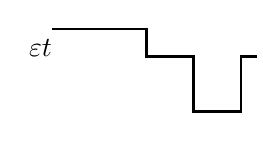
\begin{tikzpicture}\gaxesPN{$\varepsilon$}{$t$}
    \draw[line width=1pt] (0,0.35) -- (1.2,0.35) -- (1.2,0) -- (1.8,0) -- (1.8,-0.7) -- (2.4,-0.7) -- (2.4,0) -- (2.6,0);
  \end{tikzpicture}}
  {%
  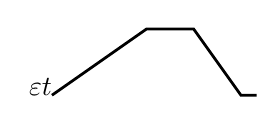
\begin{tikzpicture}\gaxesPN{$\varepsilon$}{$t$}
    \draw[line width=1pt] (0,0) -- (1.2,0.84) -- (1.8,0.84) -- (2.4,0) -- (2.6,0);
  \end{tikzpicture}}
  {%
  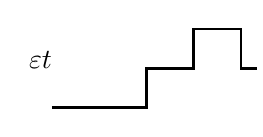
\begin{tikzpicture}\gaxesPN{$\varepsilon$}{$t$}
    \draw[line width=1pt] (0,-0.5) -- (1.2,-0.5) -- (1.2,0) -- (1.8,0) -- (1.8,0.5) -- (2.4,0.5) -- (2.4,0) -- (2.6,0);
  \end{tikzpicture}}
\end{quizq}

% ---- Q41 (loop moving away from a long wire)
\Needspace{40\baselineskip}
\begin{quizq}{}
A square loop of wire moves away at a constant speed from a long straight wire that carries a
constant current $I$. The loop stays in the same plane as the wire.
\begin{center}
  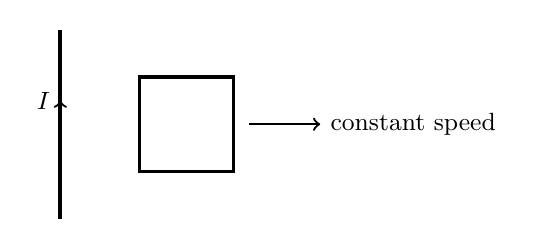
\begin{tikzpicture}
    \draw[line width=1.5pt] (0,0) -- (0,2.4); \draw[->, line width=0.8pt] (0,0.9) -- (0,1.5) node[left, font=\small] {$I$};
    \draw[line width=1.1pt] (1.0,0.6) rectangle (2.2,1.8);
    \draw[->, line width=0.8pt] (2.4,1.2) -- (3.3,1.2) node[right, font=\small] {constant speed};
  \end{tikzpicture}
\end{center}
Which graph best shows the size of the emf induced in the loop as time passes?
\gridopts{%
  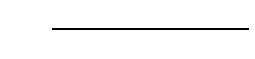
\begin{tikzpicture}\gaxesP{$\varepsilon$}{$t$}
    \draw[line width=1pt] (0,1.0) -- (2.5,1.0);
  \end{tikzpicture}}
  {%
  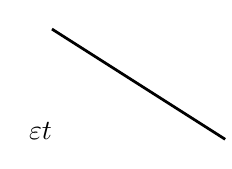
\begin{tikzpicture}\gaxesP{$\varepsilon$}{$t$}
    \draw[line width=1pt] (0,1.4) -- (2.2,0);
  \end{tikzpicture}}
  {%
  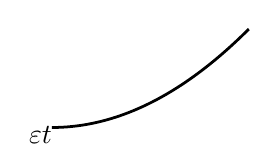
\begin{tikzpicture}\gaxesP{$\varepsilon$}{$t$}
    \draw[line width=1pt, domain=0:2.5, samples=40, smooth] plot (\x, {0.2+0.5*\x*\x/2.5});
  \end{tikzpicture}}
  {%
  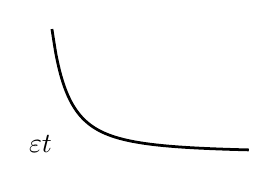
\begin{tikzpicture}\gaxesP{$\varepsilon$}{$t$}
    \draw[line width=1pt, domain=0:2.5, samples=50, smooth] plot (\x, {0.33/((0.3+\x)*(0.7+\x))});
  \end{tikzpicture}}
\end{quizq}

% ---- Q42 (Lenz's law: magnet moving away)
\Needspace{28\baselineskip}
\begin{quizq}{}
The north pole of a bar magnet is pulled away from the right-hand end of a coil, which is connected to
a galvanometer.
\begin{center}
  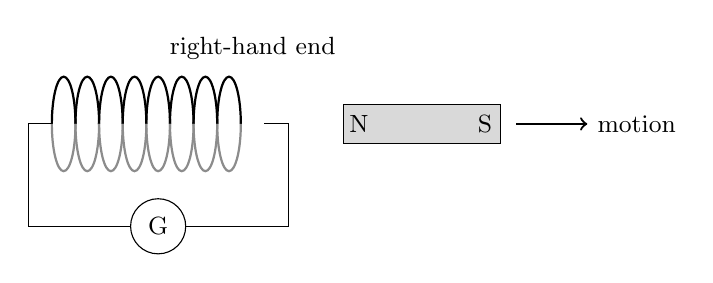
\begin{tikzpicture}
    \foreach \x in {0,0.3,...,2.4} \draw[line width=0.8pt] (\x,0) arc (180:0:0.15 and 0.6) ;
    \foreach \x in {0,0.3,...,2.4} \draw[line width=0.8pt, black!45] (\x,0) arc (180:360:0.15 and 0.6);
    \node[above, font=\small] at (2.55,0.7) {right-hand end};
    \draw (0,0) -- (-0.3,0) -- (-0.3,-1.3) -- (1.0,-1.3); \draw (1.35,-1.3) circle (0.35) node[font=\small] {G}; \draw (1.7,-1.3) -- (3.0,-1.3) -- (3.0,0) -- (2.7,0);
    \draw[fill=black!15] (3.7,-0.25) rectangle (5.7,0.25); \node[font=\small] at (3.9,0) {N}; \node[font=\small] at (5.5,0) {S};
    \draw[->, line width=0.8pt] (5.9,0) -- (6.8,0) node[right, font=\small] {motion};
  \end{tikzpicture}
\end{center}
Which row of the table correctly describes the right-hand end of the coil and the force between the
coil and the magnet while the magnet moves away?
\begin{center}
  \renewcommand\arraystretch{1.7}
  \begin{tabular}{@{}p{10mm}|>{\centering\arraybackslash}p{56mm}|>{\centering\arraybackslash}p{44mm}|}
    \cline{2-3}
    & \textit{Right-hand end of the coil acts as a} & \textit{Force on the magnet}\\ \cline{2-3}
    A. & north pole & repulsion\\ \cline{2-3}
    B. & north pole & attraction\\ \cline{2-3}
    C. & south pole & repulsion\\ \cline{2-3}
    D. & south pole & attraction\\ \cline{2-3}
  \end{tabular}
\end{center}
\end{quizq}

% ---- Q43 (two coils on an iron rod)
\Needspace{30\baselineskip}
\begin{quizq}{}
Two separate coils are wound on the same iron rod. The first coil is connected to a battery and a
switch. The second coil is connected to a galvanometer.
\begin{center}
  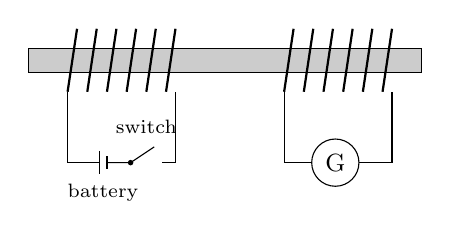
\begin{tikzpicture}
    \draw[fill=black!20] (0,-0.15) rectangle (5,0.15);
    \foreach \x in {0.5,0.75,...,1.75} \draw[line width=0.8pt] (\x,-0.4) -- (\x+0.12,0.4);
    \foreach \x in {3.25,3.5,...,4.5} \draw[line width=0.8pt] (\x,-0.4) -- (\x+0.12,0.4);
    \draw (0.5,-0.4) -- (0.5,-1.3) -- (0.9,-1.3); \draw (0.9,-1.15) -- (0.9,-1.45); \draw (1.0,-1.22) -- (1.0,-1.38); \draw (1.0,-1.3) -- (1.3,-1.3) -- (1.6,-1.1); \fill (1.3,-1.3) circle (1pt); \draw (1.7,-1.3) -- (1.87,-1.3) -- (1.87,-0.4);
    \node[below, font=\scriptsize] at (0.95,-1.45) {battery}; \node[above, font=\scriptsize] at (1.5,-1.05) {switch};
    \draw (3.25,-0.4) -- (3.25,-1.3) -- (3.6,-1.3); \draw (3.9,-1.3) circle (0.3) node[font=\small] {G}; \draw (4.2,-1.3) -- (4.62,-1.3) -- (4.62,-0.4);
  \end{tikzpicture}
\end{center}
When the switch is closed, the galvanometer needle flicks briefly to the left, then returns to zero.
Which row describes the galvanometer while the switch stays closed, and when the switch is then
opened?
\begin{center}
  \renewcommand\arraystretch{1.7}
  \begin{tabular}{@{}p{10mm}|>{\centering\arraybackslash}p{50mm}|>{\centering\arraybackslash}p{50mm}|}
    \cline{2-3}
    & \textit{While the switch stays closed} & \textit{When the switch is opened}\\ \cline{2-3}
    A. & Stays to the left & Flicks briefly to the right\\ \cline{2-3}
    B. & Reads zero & Flicks briefly to the left\\ \cline{2-3}
    C. & Reads zero & Flicks briefly to the right\\ \cline{2-3}
    D. & Stays to the left & Reads zero\\ \cline{2-3}
  \end{tabular}
\end{center}
\end{quizq}

% ---- Q44 (loop with a lamp moving through a field region)
\Needspace{26\baselineskip}
\begin{quizq}{}
A loop of wire containing a small lamp moves at a constant speed to the right, through a region of
uniform magnetic field. The region is wider than the loop.
\begin{center}
  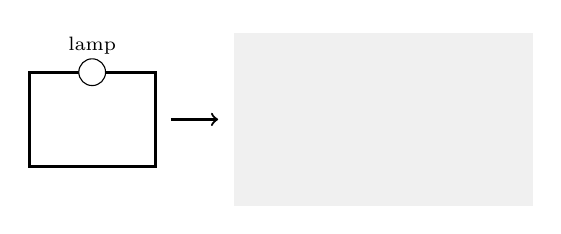
\begin{tikzpicture}
    \fill[black!6] (2.6,-0.3) rectangle (6.4,1.9); \fieldin{2.8}{-0.1}{6.2}{1.8}{0.45}
    \draw[line width=1.1pt] (0,0.2) rectangle (1.6,1.4); \draw[fill=white] (0.8,1.4) circle (0.17); \node[above=3pt, font=\scriptsize] at (0.8,1.4) {lamp};
    \draw[->, line width=0.8pt] (1.8,0.8) -- (2.4,0.8);
  \end{tikzpicture}
\end{center}
When does the lamp light up?
\opts{During the whole time the loop is moving}{Only while the loop is completely inside the field}
  {Never, because the speed of the loop is constant}{Only while the loop is entering and while it is
  leaving the field}
\end{quizq}

% ---- Q45 (rotating rod: emf in two arrangements)
\Needspace{22\baselineskip}
\begin{quizq}{}
A metal rod rotates at a constant rate about one of its ends, in a uniform magnetic field. In
arrangement 1, the field is at right angles to the plane in which the rod rotates. In arrangement 2,
the field lies in the plane in which the rod rotates. Which row describes the emf between the ends of
the rod?
\begin{center}
  \renewcommand\arraystretch{1.7}
  \begin{tabular}{@{}p{10mm}|>{\centering\arraybackslash}p{50mm}|>{\centering\arraybackslash}p{50mm}|}
    \cline{2-3}
    & \textit{Arrangement 1} & \textit{Arrangement 2}\\ \cline{2-3}
    A. & Constant, not zero & Zero\\ \cline{2-3}
    B. & Zero & Constant, not zero\\ \cline{2-3}
    C. & Constant, not zero & Constant, not zero\\ \cline{2-3}
    D. & Changes as the rod rotates & Zero\\ \cline{2-3}
  \end{tabular}
\end{center}
\end{quizq}

% ---- Q46 (rod sliding on rails)
\Needspace{28\baselineskip}
\begin{quizq}{}
A metal rod of length \qty{0.50}{m} slides at \qty{2.0}{m.s^{-1}} along two parallel metal rails in a
uniform magnetic field of \qty{0.30}{T}, directed into the page. The rails are joined by a
\qty{1.5}{\ohm} resistor.
\begin{center}
  \begin{tikzpicture}
    \fieldin{0.5}{0.25}{4.5}{1.75}{0.5}
    \draw[line width=1pt] (0,0) -- (5,0); \draw[line width=1pt] (0,2) -- (5,2);
    \draw (0,0) -- (0,0.6); \draw[fill=white] (-0.15,0.6) rectangle (0.15,1.4); \draw (0,1.4) -- (0,2); \node[left, font=\small] at (-0.15,1.0) {\qty{1.5}{\ohm}};
    \draw[line width=2pt] (3.2,0) -- (3.2,2); \draw[->, line width=0.9pt] (3.2,2.45) -- (4.1,2.45) node[right, font=\small] {\qty{2.0}{m.s^{-1}}};
    \draw[|<->|, line width=0.4pt] (5.5,0) -- (5.5,2) node[midway, right, font=\small] {\qty{0.50}{m}};
  \end{tikzpicture}
\end{center}
What is the current in the resistor?
\opts{\qty{0.10}{A}}{\qty{0.20}{A}}{\qty{0.40}{A}}{\qty{0.45}{A}}
\end{quizq}

% ---- Q47 (magnet falling through a copper tube)
\Needspace{16\baselineskip}
\begin{quizq}{}
A strong magnet is dropped down a vertical copper tube. An identical magnet is dropped down a plastic
tube of the same size. Which statement is correct?
\opts{Both magnets take the same time to fall, because copper is not magnetic.}
  {The magnet in the copper tube falls faster, because the induced currents attract it downwards.}
  {The magnet in the copper tube falls more slowly, because the induced currents in the tube oppose its
  motion.}
  {The magnet in the copper tube sticks to the tube, because copper is attracted to magnets.}
\end{quizq}

% ---- Q48 (transformer turns)
\Needspace{12\baselineskip}
\begin{quizq}{}
An ideal transformer changes \qty{240}{V} AC to \qty{12}{V} AC. Its primary coil has 1200 turns. How many
turns are on the secondary coil?
\opts{5}{60}{2400}{\num{24000}}
\end{quizq}

% ---- Q49 (type of transformer from the currents)
\Needspace{20\baselineskip}
\begin{quizq}{}
In an ideal transformer, the current in the secondary coil is 5 times the current in the primary
coil. Which row of the table correctly describes the transformer?
\begin{center}
  \renewcommand\arraystretch{1.7}
  \begin{tabular}{@{}p{10mm}|>{\centering\arraybackslash}p{45mm}|>{\centering\arraybackslash}p{60mm}|}
    \cline{2-3}
    & \textit{Type of transformer} & \textit{Turns ratio $N_\mathrm{p} : N_\mathrm{s}$}\\ \cline{2-3}
    A. & Step-up & $1 : 5$\\ \cline{2-3}
    B. & Step-up & $5 : 1$\\ \cline{2-3}
    C. & Step-down & $5 : 1$\\ \cline{2-3}
    D. & Step-down & $1 : 5$\\ \cline{2-3}
  \end{tabular}
\end{center}
\end{quizq}

% ---- Q50 (doubling the output voltage)
\Needspace{13\baselineskip}
\begin{quizq}{}
The input voltage to an ideal transformer stays the same. Which change would double the output
voltage?
\opts{Doubling the number of turns on the primary coil}{Halving the number of turns on the primary
  coil}{Doubling the number of turns on both coils}{Halving the number of turns on the secondary coil}
\end{quizq}

% ---- Q51 (transmission of electrical energy)
\Needspace{16\baselineskip}
\begin{quizq}{}
Which statement correctly describes how electrical energy is transmitted from a power station to
homes?
\opts{The voltage is stepped down at the power station so the current is large, then stepped up for
   homes.}
  {The voltage is kept the same, because transformers waste energy.}
  {The voltage is stepped up at the power station so the current is large, which reduces energy loss.}
  {The voltage is stepped up at the power station so the current is small, then stepped down near the
   homes.}
\end{quizq}

% ---- Q52 (power loss in a transmission line)
\Needspace{13\baselineskip}
\begin{quizq}{}
A power station sends \qty{50}{MW} along a transmission line of total resistance \qty{5.0}{\ohm}, at a
voltage of \qty{250}{kV}. What is the power lost as heat in the line?
\opts{\qty{1.0e3}{W}}{\qty{2.0e5}{W}}{\qty{2.0e7}{W}}{\qty{1.25e10}{W}}
\end{quizq}

% ---- Q53 (laminated core)
\Needspace{16\baselineskip}
\begin{quizq}{}
The iron core of a real transformer is made of thin sheets (laminations) that are insulated from each
other. Why does this improve the efficiency of the transformer?
\opts{It reduces the eddy currents in the core, so less energy is lost as heat.}
  {It increases the resistance of the coils, so less current flows.}
  {It stops all of the magnetic flux from leaving the core.}
  {It makes the core lighter, so it vibrates less.}
\end{quizq}

% ---- Q54 (DC into a transformer)
\Needspace{13\baselineskip}
\begin{quizq}{}
A \qty{12}{V} battery is connected to the primary coil of a step-up transformer with a turns ratio
of $1 : 10$. What is the output voltage once the current in the primary coil is steady?
\opts{\qty{0}{V}}{\qty{1.2}{V}}{\qty{12}{V}}{\qty{120}{V}}
\end{quizq}
